\documentclass[conference]{IEEEtran}
\IEEEoverridecommandlockouts
\usepackage{cite}
\usepackage{amsmath,amssymb,amsfonts}
\usepackage{algorithmic}
\usepackage{graphicx}
\usepackage{textcomp}
\usepackage{xcolor}
\usepackage{float}
\usepackage{graphicx}

\floatstyle{boxed} 
\restylefloat{figure}

\def\BibTeX{{\rm B\kern-.05em{\sc i\kern-.025em b}\kern-.08em
    T\kern-.1667em\lower.7ex\hbox{E}\kern-.125emX}}
\begin{document}

\title{Report: Sleep State Prediction Using Accelerometry Data}

\author{
	\IEEEauthorblockN{Juan Carlos Quintero Rubiano}
	\IEEEauthorblockA{Code: 20232020172\\
		\textit{Systems Engineering} \\
		\textit{Francisco Jose de Caldas District University}\\
		Bogota, Colombia \\
		jcquineror@udistrital.edu.co}\\
	\IEEEauthorblockN{Juan Felipe Wilches Gomez}
	\IEEEauthorblockA{Code: 20231020137\\
		\textit{Systems Engineering} \\
		\textit{Francisco Jose de Caldas District University}\\
		Bogota, Colombia \\
		jfwilchesg@udistrital.edu.co}
	\and
	\IEEEauthorblockN{Juan Nicolas Diaz Salamanca}
	\IEEEauthorblockA{Code: 20232020059\\
		\textit{Systems Engineering} \\
		\textit{Francisco Jose de Caldas District University}\\
		Bogota, Colombia \\
		jndiazs@udistrital.edu.co}
}

\maketitle

\begin{abstract}
	The study of sleep is crucial for diagnosing sleep disorders; however, the traditional method, polysomnography (PSG), is costly and impractical for long-term use. This paper presents a systematic computational approach to predict sleep states using accelerometry data from low-cost, non-invasive wrist-worn devices. Movement patterns (ENMO, Anglez) are analyzed through a five-stage pipeline: acquisition, preprocessing, feature extraction, classification, and validation.
\end{abstract}

\section{Introduction}

Sleep constitutes a complex physiological process subdivided into distinct stages: wakefulness, light sleep (N1, N2), deep sleep (N3), and REM sleep.

Polysomnography (PSG) remains the gold standard in sleep analysis due to its high reliability and granular data acquisition. Nevertheless, its prohibitive cost and confinement to specialized clinical environments render it unsuitable for longitudinal sleep monitoring.

Wearable accelerometers, through movement analysis, provide a non-invasive, cost-effective, and accessible alternative. However, their precision in discerning specific sleep stages remains inferior to PSG, as they lack neurophysiological inputs such as cerebral activity (EEG), muscular tone (EMG), or ocular movements (EOG). Despite this limitation, accelerometers demonstrate robust performance in binary sleep/wake classification.

This computational framework underscores accelerometry's potential for large-scale sleep surveillance and personalized health tracking, while acknowledging persistent challenges such as inter-individual variability, microarousal detection, and temporal-context dependency.


\section{Metodology}

The proposed model adheres to a meticulously structured five-stage processing pipeline:
\subsection{Data}
\begin{itemize}
	\item \textbf{Source of Data:}
	      Triaxial accelerometers embedded in wrist-worn wearables.
	\item \textbf{Key Variables:}
	      \begin{itemize}
		      \item \textbf{Enmo:}  Normalized and filtered vertical acceleration (m/s²).
		      \item \textbf{Anglez:} Static-position-derived wrist angle relative to the body.
                \item \textbf{TimeStamp:} Temporal indexing for circadian rhythm analysis.
	      \end{itemize}
\end{itemize}
\subsection{Processing Pipeline}

\begin{figure}[h]
    \centering
    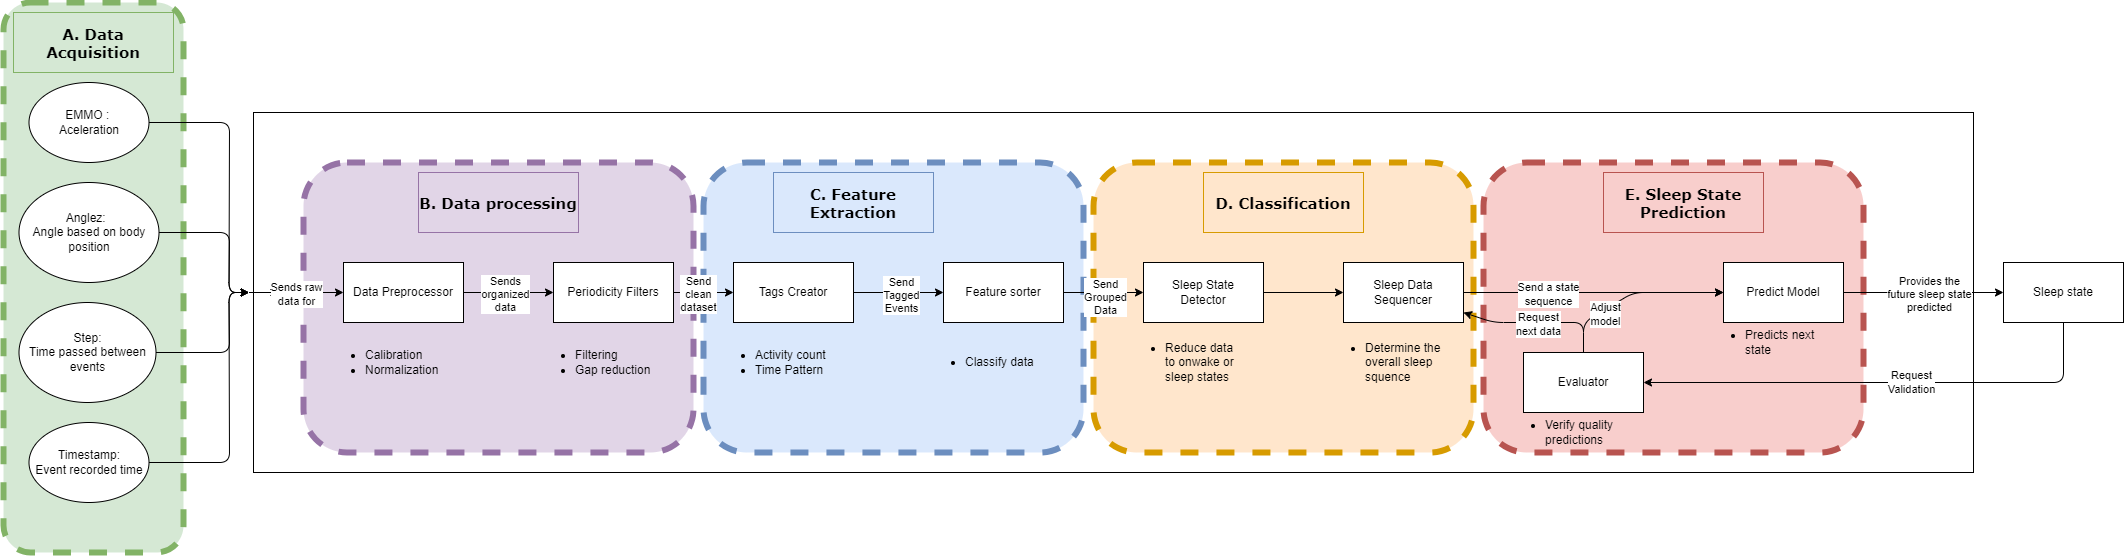
\includegraphics[width=\linewidth]{conceptual_model.png}
    \caption{Expanded conceptual model of sleep state classification using accelerometer data. ...}
    \label{fig:conceptual_model}
\end{figure}

\begin{itemize}
	\item \textbf{Acquisition:}
	      Capture of raw triaxial accelerometric signals.
	\item \textbf{Preprocessing:}
            \begin{itemize}
		      \item \textbf{Filtering:} Attenuation of high-frequency noise (abrupt motion artifacts) via low-pass filters.
              
		      \item \textbf{Normalization:} Feature scaling to mitigate inter-subject variability.
                \item \textbf{Missing Data Imputation:} Linear interpolation or k-nearest neighbors (KNN)-based statistical imputation.
	      \end{itemize}
    \item \textbf{Feature Extraction:}
            \begin{itemize}
		      \item \textbf{Time-Domain Features:}
                    \begin{itemize}
		              \item \textbf{Raw Activity Counts:}  Summated acceleration differentials within 30-second windows.
		              \item \textbf{Movement Variability:} Signal entropy and standard deviation quantification.
                        \item \textbf{Inactivity Duration:} Consecutive motionless intervals.
	               \end{itemize}
		      \item \textbf{Frequency-Domain Features:}
                    \begin{itemize}
                        \item \textbf{Spectral Power Density:} Fourier analysis to identify rhythmic patterns (REM movements).
                    \end{itemize}
                \item \textbf{Tagged Events:} Identification of transitions from wakefulness to sleep based on movement thresholds.
	      \end{itemize}
    \item \textbf{Clasification:}
            \begin{itemize}
		      \item \textbf{Threshold Based Algorithms:}
                    \begin{itemize}
                        \item \textbf{Sadeh:} It ponders activity in 11-minute windows, commonly used with children and adolescents.
                        \item \textbf{Cole-Kripke:} Pondering algorithm similar to Sadeh but more targeted at the adult population.
                    \end{itemize}
                \item \textbf{Machine Learning Models:}
                     \begin{itemize}
                        \item \textbf{Random Forest} 
                        \item \textbf{SVM} 
                    \end{itemize}
                \item \textbf{Deep Learning:}
                    \begin{itemize}
                        \item \textbf{LSTM} 
                        \item \textbf{CNN}
                        \item \textbf{TCN} 
                    \end{itemize}
	      \end{itemize}
    \item \textbf{Prediction and Validation:}
            \begin{itemize}
		      \item \textbf{Predictive Model:} Estimation of the next sleep state according to historical sequences.
		      \item \textbf{Evaluation:} Comparison with PSG, using metrics.
                \item \textbf{Cohen Kappa:} Values between 0.55 and 0.80 are reported in valitadion studies, this means moderate to substantial agreement with polysomnography (PSG). 
                \item \textbf{F1 Score:} Ranges from 0.81 to 0.90 in recent studies using advanced algorithms.
	      \end{itemize}
    
\end{itemize}

\section{Key Results}

\subsection{Model Performance}
    The models Sadeh, Cole Kripke, Random Forest, LSTM, were evaluated across multiple studies:
    
\begin{table}[h]
\centering
\small
\begin{tabular}{|p{0.9cm}|c|c|c|c|}
\hline
\textbf{Model} & \textbf{Accuracy} & \textbf{Sensitivity} & \textbf{Especificity} & \textbf{Kappa} \\
\hline
\textbf{Sadeh Cole-Kripke} & 82--87\% & 87--90\% & 52--77\% & 0.55--0.70 \\
\hline
\textbf{Random Forest} & 87--91\% & 89--93\% & 69--80\% & 0.65--0.75 \\
\hline
\textbf{LSTM} & 85--92\% & 90--95\% & 75--83\% & 0.70--0.80 \\
\hline
\end{tabular}
\caption{Comparative Performance of Sleep State Prediction Models}
\label{tab:modelos}
\end{table}

\begin{itemize}
	\item \textbf{Binary Classification (Sleep/Wake):}
	      \begin{itemize}
		      \item Accelerometers are highly effective, showing maximum performance with LSTM (92% accuracy).
		      \item Main limitation being a higher percentage of error in micro-awakenings (50-60% detection).
	      \end{itemize}
	\item \textbf{Distinction of stages:}
	      \begin{itemize}
		      \item Deep Sleep (N3): Identified with 65-70\% accuracy using patterns of prolonged inactivity.
		      \item REM: Difficult to distinguish from wakefulness (<60\% accuracy due to lack of EOG/EMG signals).
	      \end{itemize}
\end{itemize}

\subsection{Comparison between PSG and Accelerometry}
    The next table shows PSG compared to accelerometry in costs, environment ,stages, invasiveness and temporary resolution

\begin{table}[h]
\centering
\small
\begin{tabular}{|p{1.4cm}|p{3.0cm}|p{3.4cm}|}
\hline
\textbf{Aspect} & \textbf{PSG} & \textbf{Accelerometry} \\
\hline
\textbf{Environment} & Lab & Anywhere \\
\hline
\textbf{Cost per night} & >\$1000 & <\$200 (commercial device) \\
\hline
\textbf{Stages detected} & 5 (Wake, N1, N2, N3, REM) & 2--3 (Wake, Sleep; N3 in some cases) \\
\hline
\textbf{Invasiveness} & High (electrodes on the body) & Non invasive \\
\hline
\textbf{Temporary resolution} & 30 seconds per session & 1--5 minutes per session \\
\hline
\end{tabular}
\caption{Comparison between PSG and Accelerometry}
\label{tab:psg-vs-acelerometry}
\end{table}

\section{Advantages and Limitations}

The use of accelerometry promises to be non-invasive and cost-effective; however, as an indirect measurement method, it has strengths and limitations that must be considered when interpreting its results.

\subsection{Advantages}

\begin{itemize}
	\item \textbf{Accessibility:} Allows long-term studies in natural environments.
	\item \textbf{Integration with Wearables:} Continuous data for personalized sleep quality monitoring.
    \item \textbf{Cost Effectiveness:} Ideal for detecting sleep disorder diseases in people without symptoms.
\end{itemize}

\subsection{Limitations}

\begin{itemize}
	\item \textbf{Lack of neurophysiological signals:} Since accelerometers only measure movement, there is no data on brain activity (EEG) or eye movements (EOG), key aspects for detecting sleep stages and especially REM sleep.
	\item \textbf{Individual variability:} 
            \begin{itemize}
		      \item General models fail in special populations such as children or patients with Parkinson's.
		      \item 5-15\% less precision is found in these groups.
	      \end{itemize}
    \item \textbf{Transitions and Microawakenings:} 
            \begin{itemize}
		      \item 78\% of errors occur in the first 5 minutes of state changes.
		      \item Microawakenings shorter than 30 seconds are underestimated.
	      \end{itemize}
\end{itemize}

\section{Conclusions: }
    
    \begin{itemize}
		\item Accelerometers are valid tools for binary sleep/wake classification, with accuracy comparable to PSG in this area. (90\% in advanced models).
        \item \textbf{Future directions:} 
        \begin{itemize}
		      \item \textbf{Hybrid Models:} Combining accelerometry with multimodal biometrics like PPG for heart rate variability or temperature sensors to approximate performance to that of PSG. Early studies suggest hybrid systems could achieve 80-85\% accuracy in N3 and REM identification.
                \item \textbf{Hybrid architectures:} Hybrid architectures that fuse LSTM and CNN show potential in addressing transitional ambiguity. However micro wakings detection remains an unsolved challenge.
		      \item \textbf{Personalization:} There is a need to train algorithms with individual data to reduce errors because of variability, due to a reduce in performance in atypical populations (5-15\% accuracy loss in children).
                \item \textbf{Clinical Applications:} Clinical validation for the commercialization of wearables for public use, so that they can be used to diagnose insomnia, sleep apnea, or monitor treatments or medications that affect sleep quality.
                \item \textbf{Clinical Limitations:} Accelerometry remains insufficient for diagnosing complex sleep disorders that require a detailed analysis of the stages such as narcolepsy, REM sleep behavior disorder, circadian rhythm disturbances. Polysomnography (PSG) remains irreplaceable in neurology and sleep medicine despite its disadvantages.
	      \end{itemize}
	\end{itemize}

\end{document}